\begin{frame}
  \frametitle{Strada per la dimostrazione del teorema di BB}
  \begin{enumerate}
    \item Dato $(Z,d)$ spazio metrico completo e limitato, si può costruire uno spazio Gromov-iperbolico $\big(\text{Con}(Z),r\big)$ tale che $Z$ è identificato con il bordo.
    \pause
    \item La metrica di Kobayashi soddisfa una particolare catena di disuguaglianze; \pause usando tali disuguaglianze si può dimostrare che $k_{\Omega}$, vicino al bordo, differisce per una costante da una certa funzione $g$ che è sostanzialmente l'equivalente di $r$ per $\Omega$ (si dice che $k_{\Omega}$ e $g$ sono quasi-isometriche).
    \pause
    \item Poiché la Gromov-iperbolicità è invariante per quasi-isometrie, questo ci permette di dire che $(\Omega,k_{\Omega})$ è Gromov-iperbolico.
  \end{enumerate}
\end{frame}

\begin{frame}[t]
  \frametitle{1. Lo spazio iperbolico $\text{Con}(Z)$}
  \only<1-4>{
  \begin{block}{Teorema (Bonk-Schramm, 2000)}\begin{itshape}
    Sia $(Z,d)$ uno spazio metrico completo e limitato, e sia $\text{Con}(Z)=Z\times(0, D(Z)]$, dove $D(Z)$ è il diametro di $Z$.
    La funzione $r:\text{Con}(Z)\times\text{Con}(Z) \longrightarrow [0,+\infty)$ data da
    $$r\big((z,h),(z',h')\big)=2\log\left(\frac{d(z,z')+\max\{h, h'\}}{\sqrt{hh'}}\right)$$
    è una distanza su $\text{Con}(Z)$ che lo rende uno spazio Gromov-iperbolico, il cui bordo può essere identificato con $Z$.
  \end{itshape}\end{block}
  }
  \only<2-4>{
  \textit{Traccia della dimostrazione:} è facile verificare che $r$ è una distanza.

  }
  \only<3-4>{Dati $r_{ij} \ge 0$ per $i,j \in \{1,2,3,4\}$ tali che $r_{ij}=r_{ji}$ e $r_{ij} \le r_{ik}+r_{kj}$, allora $r_{12}r_{34} \le 4\cdot\max\{r_{13}r_{24}, r_{14}r_{23}\}$.

  }
  \only<4>{
  Poniamo $x_i=(z_i,h_i) \in \text{Con}(Z)$ per $i \in \{1,2,3,4\}$, $d_{ij}=d(z_i,z_j)$ e $r_{ij}=d_{ij}+\max\{h_i, h_j\}$.
  }
  \only<5-6>{Segue che
  \begin{align*}
    (d_{12}+\max\{h_1, h_2\}&)(d_{34}+\max\{h_3, h_4\}) \\
    &\le 4\Big(\big((d_{13}+\max\{h_1, h_3\})(d_{24}+\max\{h_2, h_4\})\big) \\
    &\times\big((d_{14}+\max\{h_1, h_4\})(d_{23}+\max\{h_2, h_3\})\big)\Big),
  \end{align*}}
  \only<6>{che ci dà
  \begin{gather*}
    r(x_1,x_2)+r(x_3,x_4) \le \big(r(x_1,x_3)+r(x_2,x_4)\big)\big(r(x_1,x_4)+r(x_2,x_3)\big)+C,
  \end{gather*}
  da cui segue la Gromov-iperbolicità di $\big(\textit{Con}(Z), r\big)$.}
  \only<7->{
  Fissiamo $w=\big(z_0,D(Z)\big) \in \text{Con}(Z)$; usando le definizioni, troviamo che dati $x=(z,h),x'=(z',h')\in \text{Con}(Z)$ vale
  $$(x,x')_w=-\log\big(d(z,z')+\max\{h, h'\}\big)+O_{D(Z)}(1).$$}
  \only<8->{Segue che una successione $(x_i)$ in $\big(\text{Con}(Z),r\big)$ converge a infinito se e solo se la successione $(z_i)$ è di Cauchy e $h_i \longrightarrow 0$; essendo $Z$ completo, possiamo quindi associare a $(x_i)$, come ``limite'', un unico $z \in Z$.}
  \only<9->{
  Inoltre, due successioni convergenti a infinito sono equivalenti se e solo se il loro limite è lo stesso, e ogni punto di $Z$ è limite di una successione che converge a infinito; questo ci dà un'identificazione, come insiemi, di $Z$ e $\partial_G\text{Con}(Z)$.

  }
  \only<10->{
  Mettendo su $\text{Con}(Z)\cup\partial_G\text{Con}(Z)$ un'opportuna topologia (di compattificazione), segue anche che $Z$ e $\partial_G\text{Con}(Z)$ sono identificati come spazi topologici; \only<11>{questo non è difficile, ma richiede un po' di passaggi che non vedremo. \qed}
  }
\end{frame}

\begin{frame}[t]
  \frametitle{Intorno tubolare e tangente ortogonale complesso}
  \only<1->{
  Sia $N_{\epsilon}(\partial\Omega)=\{x \in \mathbb{C}^n \mid \delta(x)<\epsilon\}$. Si può dimostrare che esiste $\epsilon>0$ tale che $N_{\epsilon}(\partial\Omega)$ è un intorno tubolare di $\partial\Omega$.
  }
  \only<2->{
  \begin{center}
    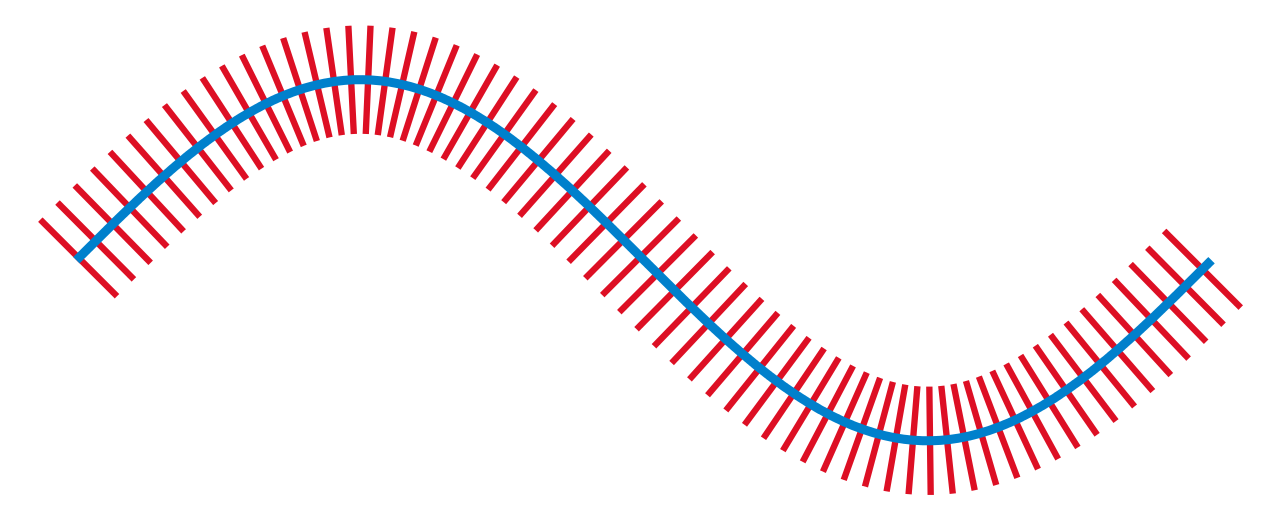
\includegraphics[width=0.36\textwidth]{intornotubolare.png}
  \end{center}
  }
  \only<3->{
  Sia $\pi$ la proiezione su $\partial\Omega$; dati $x,y \in \Omega\cap N_{\epsilon}(\partial\Omega)$, poniamo
  $$g(x,y)=2\log\left(\frac{d_H\big(\pi(x),\pi(y)\big)+\max\{\delta(x)^{1/2 },\,\delta(y)^{1/2}\}}{\sqrt{\delta(x)^{1/2 }\delta(y)^{1/2}}}\right).$$
  }
  \only<4>{
  Fissato $p \in \partial\Omega$ e detta $\nu(p)$ la normale reale uscente da $\partial\Omega$ in $p$, possiamo decomporre $\mathbb{C}^n=H_p\partial\Omega\oplus \text{Span}_{\mathbb{C}}\{\nu(p)\}$;
  dato $Z \in \mathbb{C}^n$, scriviamo in modo unico $Z=Z_H+Z_N$ con $Z_H \in H_p\partial\Omega$ e $Z_N \in \text{Span}_{\mathbb{C}}\{\nu(p)\}$.
  }
\end{frame}

\begin{frame}[t]
  \frametitle{2. Stime per la metrica di Kobayashi}
  \only<1->{\begin{prop}
    Per ogni $\epsilon>0$ esistono $\epsilon_0>0$ e $C \ge 0$ tali che per ogni $x \in \Omega\cap N_{\epsilon_0}(\partial\Omega)$ e per ogni $Z \in \mathbb{C}^n$ si ha
    \begin{multline*}
      \big(1-C\delta^{1/2}(x)\big)\left(\frac{|Z_N|^2}{4\delta^2(x)}+(1-\epsilon)\frac{L_\rho\big(\pi(x);Z_H\big)}{\delta(x)}\right)^{1/2} \le K_{\Omega}(x;Z) \\
      \le \big(1+C\delta^{1/2}(x)\big)\left(\frac{|Z_N|^2}{4\delta^2(x)}+(1+\epsilon)\frac{L_\rho\big(\pi(x);Z_H\big)}{\delta(x)}\right)^{1/2}.
    \end{multline*}
  \end{prop}}
  \only<2-4>{\textit{Traccia della dimostrazione:} si localizza a un intorno di un punto del bordo.}\only<3-4>{ Con un opportuno biolomorfismo, ci si sposta in un insieme che può essere stretto fra due ellissoidi complessi, uno contenuto e uno che lo contiene.}\only<4>{ Per gli ellissoidi complessi, la metrica di Kobayashi può essere calcolata esplicitamente. \qed}
\end{frame}

\begin{frame}[t]
  \frametitle{2. Vicino al bordo, $k_{\Omega}$ e $g$ sono quasi-isometriche}
  \only<1->{
  \begin{thm}
    Sia $\Omega$ un dominio strettamente pseudoconvesso limitato, e sia $k_{\Omega}$ la distanza di Kobayashi su $\Omega$. Allora esiste $C \ge 0$ tale che per ogni $x, y \in \Omega$ vale
    \begin{equation} \label{stimadistanzakobayashi}
      g(x,y)-C \le k_{\Omega}(x,y) \le g(x,y)+C.
    \end{equation}
  \end{thm}
  }
  \only<2-3>{
  \textit{Idea della dimostrazione:} per la maggiorazione, si cercano delle curve che siano quasi-geodetiche, cioè che realizzano la distanza a meno di una costante additiva, e si integra lungo quelle curve.
  }
  \only<3>{

  Per la minorazione, bisogna mostrare che la stima trovata dall'alto è ottimale, cioè che vale la stima dal basso per tutte le curve.
  }
  \only<4>{
  3. Come già osservato, l'invarianza della Gromov-iperbolicità per quasi-isometrie ci permette di ottenere come corollario il teorema di Balogh-Bonk.
  }
\end{frame}
